\chapter{The Prison Register}

The day after that in which the scene we have just described had taken
place on the road between Bellegarde and Beaucaire, a man of about
thirty or two-and-thirty, dressed in a bright blue frock coat, nankeen
trousers, and a white waistcoat, having the appearance and accent of an
Englishman, presented himself before the mayor of Marseilles.

“Sir,” said he, “I am chief clerk of the house of Thomson \& French, of
Rome. We are, and have been these ten years, connected with the house
of Morrel \& Son, of Marseilles. We have a hundred thousand francs or
thereabouts loaned on their securities, and we are a little uneasy at
reports that have reached us that the firm is on the brink of ruin. I
have come, therefore, express from Rome, to ask you for information.”

“Sir,” replied the mayor. “I know very well that during the last four
or five years misfortune has seemed to pursue M. Morrel. He has lost
four or five vessels, and suffered by three or four bankruptcies; but
it is not for me, although I am a creditor myself to the amount of ten
thousand francs, to give any information as to the state of his
finances. Ask of me, as mayor, what is my opinion of M. Morrel, and I
shall say that he is a man honorable to the last degree, and who has up
to this time fulfilled every engagement with scrupulous punctuality.
This is all I can say, sir; if you wish to learn more, address yourself
to M. de Boville, the inspector of prisons, No. 15, Rue de Nouailles;
he has, I believe, two hundred thousand francs in Morrel’s hands, and
if there be any grounds for apprehension, as this is a greater amount
than mine, you will most probably find him better informed than
myself.”

The Englishman seemed to appreciate this extreme delicacy, made his bow
and went away, proceeding with a characteristic British stride towards
the street mentioned.

M. de Boville was in his private room, and the Englishman, on
perceiving him, made a gesture of surprise, which seemed to indicate
that it was not the first time he had been in his presence. As to M. de
Boville, he was in such a state of despair, that it was evident all the
faculties of his mind, absorbed in the thought which occupied him at
the moment, did not allow either his memory or his imagination to stray
to the past.

The Englishman, with the coolness of his nation, addressed him in terms
nearly similar to those with which he had accosted the mayor of
Marseilles.

“Oh, sir,” exclaimed M. de Boville, “your fears are unfortunately but
too well founded, and you see before you a man in despair. I had two
hundred thousand francs placed in the hands of Morrel \& Son; these two
hundred thousand francs were the dowry of my daughter, who was to be
married in a fortnight, and these two hundred thousand francs were
payable, half on the 15th of this month, and the other half on the 15th
of next month. I had informed M. Morrel of my desire to have these
payments punctually, and he has been here within the last half-hour to
tell me that if his ship, the \textit{Pharaon}, did not come into port on the
15th, he would be wholly unable to make this payment.”

“But,” said the Englishman, “this looks very much like a suspension of
payment.”

“It looks more like bankruptcy!” exclaimed M. de Boville despairingly.

The Englishman appeared to reflect a moment, and then said, “From which
it would appear, sir, that this credit inspires you with considerable
apprehension?”

“To tell you the truth, I consider it lost.”

“Well, then, I will buy it of you!”

“You?”

“Yes, I!”

“But at a tremendous discount, of course?”

“No, for two hundred thousand francs. Our house,” added the Englishman
with a laugh, “does not do things in that way.”

“And you will pay——”

“Ready money.”

\begin{figure}[ht]
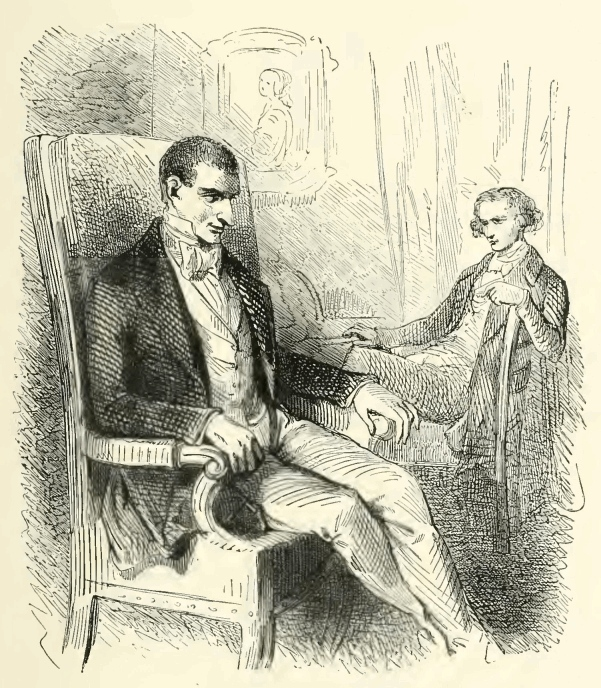
\includegraphics[width=\textwidth]{20023m.jpg}
\end{figure}

And the Englishman drew from his pocket a bundle of bank-notes, which
might have been twice the sum M. de Boville feared to lose. A ray of
joy passed across M. de Boville’s countenance, yet he made an effort at
self-control, and said:

“Sir, I ought to tell you that, in all probability, you will not
realize six per cent of this sum.”

“That’s no affair of mine,” replied the Englishman, “that is the affair
of the house of Thomson \& French, in whose name I act. They have,
perhaps, some motive to serve in hastening the ruin of a rival firm.
But all I know, sir, is, that I am ready to hand you over this sum in
exchange for your assignment of the debt. I only ask a brokerage.”

“Of course, that is perfectly just,” cried M. de Boville. “The
commission is usually one and a half; will you have two—three—five per
cent, or even more? Whatever you say.”

“Sir,” replied the Englishman, laughing, “I am like my house, and do
not do such things—no, the commission I ask is quite different.”

“Name it, sir, I beg.”

“You are the inspector of prisons?”

“I have been so these fourteen years.”

“You keep the registers of entries and departures?”

“I do.”

“To these registers there are added notes relative to the prisoners?”

“There are special reports on every prisoner.”

“Well, sir, I was educated at Rome by a poor devil of an abbé, who
disappeared suddenly. I have since learned that he was confined in the
Château d’If, and I should like to learn some particulars of his
death.”

“What was his name?”

“The Abbé Faria.”

“Oh, I recollect him perfectly,” cried M. de Boville; “he was crazy.”

“So they said.”

“Oh, he was, decidedly.”

“Very possibly; but what sort of madness was it?”

“He pretended to know of an immense treasure, and offered vast sums to
the government if they would liberate him.”

“Poor devil!—and he is dead?”

“Yes, sir, five or six months ago, last February.”

“You have a good memory, sir, to recollect dates so well.”

“I recollect this, because the poor devil’s death was accompanied by a
singular incident.”

“May I ask what that was?” said the Englishman with an expression of
curiosity, which a close observer would have been astonished at
discovering in his phlegmatic countenance.

“Oh dear, yes, sir; the abbé’s dungeon was forty or fifty feet distant
from that of one of Bonaparte’s emissaries,—one of those who had
contributed the most to the return of the usurper in 1815, a very
resolute and very dangerous man.”

“Indeed!” said the Englishman.

“Yes,” replied M. de Boville; “I myself had occasion to see this man in
1816 or 1817, and we could only go into his dungeon with a file of
soldiers. That man made a deep impression on me; I shall never forget
his countenance!”

\begin{figure}[h]
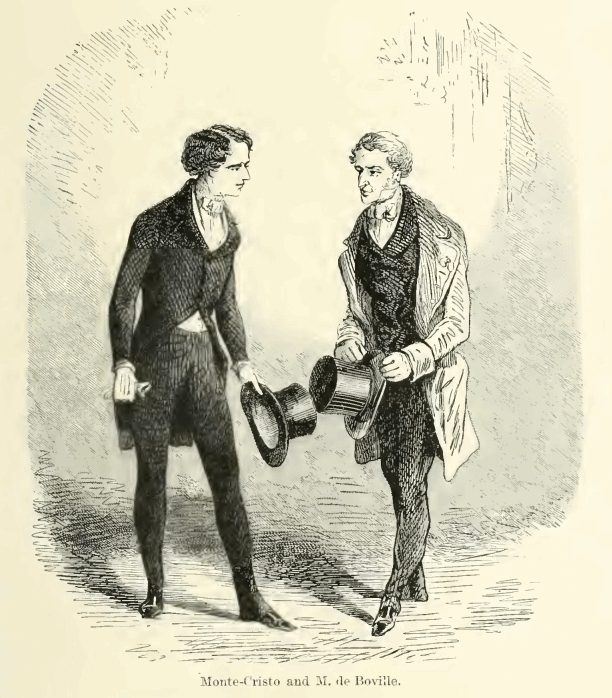
\includegraphics[width=\textwidth]{20025m.jpg}
\end{figure}

The Englishman smiled imperceptibly.

“And you say, sir,” he interposed, “that the two dungeons——”

“Were separated by a distance of fifty feet; but it appears that this
Edmond Dantès——”

“This dangerous man’s name was——”

“Edmond Dantès. It appears, sir, that this Edmond Dantès had procured
tools, or made them, for they found a tunnel through which the
prisoners held communication with one another.”

“This tunnel was dug, no doubt, with an intention of escape?”

“No doubt; but unfortunately for the prisoners, the Abbé Faria had an
attack of catalepsy, and died.”

“That must have cut short the projects of escape.”

“For the dead man, yes,” replied M. de Boville, “but not for the
survivor; on the contrary, this Dantès saw a means of accelerating his
escape. He, no doubt, thought that prisoners who died in the Château
d’If were interred in an ordinary burial-ground, and he conveyed the
dead man into his own cell, took his place in the sack in which they
had sewed up the corpse, and awaited the moment of interment.”

“It was a bold step, and one that showed some courage,” remarked the
Englishman.

“As I have already told you, sir, he was a very dangerous man; and,
fortunately, by his own act disembarrassed the government of the fears
it had on his account.”

“How was that?”

“How? Do you not comprehend?”

“No.”

“The Château d’If has no cemetery, and they simply throw the dead into
the sea, after fastening a thirty-six-pound cannon-ball to their feet.”

“Well?” observed the Englishman as if he were slow of comprehension.

“Well, they fastened a thirty-six-pound ball to his feet, and threw him
into the sea.”

“Really!” exclaimed the Englishman.

“Yes, sir,” continued the inspector of prisons. “You may imagine the
amazement of the fugitive when he found himself flung headlong over the
rocks! I should like to have seen his face at that moment.”

“That would have been difficult.”

“No matter,” replied De Boville, in supreme good-humor at the certainty
of recovering his two hundred thousand francs,—“no matter, I can fancy
it.” And he shouted with laughter.

“So can I,” said the Englishman, and he laughed too; but he laughed as
the English do, “at the end of his teeth.”

“And so,” continued the Englishman who first gained his composure, “he
was drowned?”

“Unquestionably.”

“So that the governor got rid of the dangerous and the crazy prisoner
at the same time?”

“Precisely.”

\begin{figure}[ht]
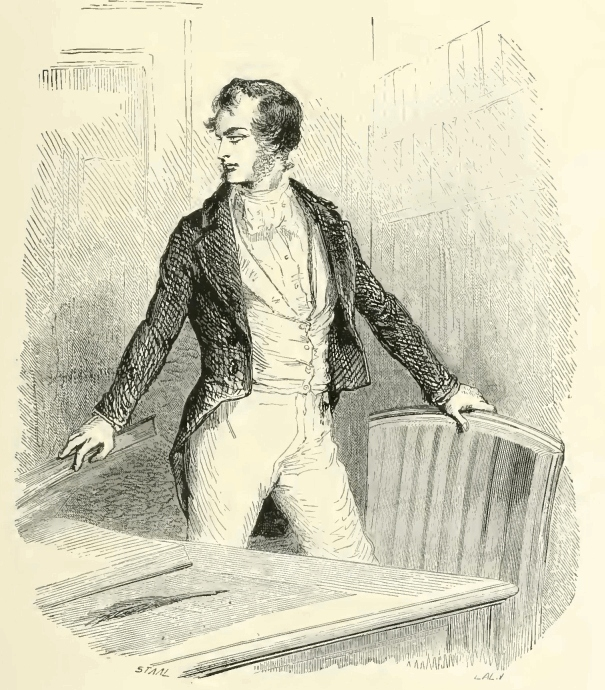
\includegraphics[width=\textwidth]{20027m.jpg}
\end{figure}

“But some official document was drawn up as to this affair, I suppose?”
inquired the Englishman.

“Yes, yes, the mortuary deposition. You understand, Dantès’ relations,
if he had any, might have some interest in knowing if he were dead or
alive.”

“So that now, if there were anything to inherit from him, they may do
so with easy conscience. He is dead, and no mistake about it.”

“Oh, yes; and they may have the fact attested whenever they please.”

“So be it,” said the Englishman. “But to return to these registers.”

“True, this story has diverted our attention from them. Excuse me.”

“Excuse you for what? For the story? By no means; it really seems to me
very curious.”

“Yes, indeed. So, sir, you wish to see all relating to the poor abbé,
who really was gentleness itself.”

“Yes, you will much oblige me.”

“Go into my study here, and I will show it to you.”

And they both entered M. de Boville’s study. Everything was here
arranged in perfect order; each register had its number, each file of
papers its place. The inspector begged the Englishman to seat himself
in an armchair, and placed before him the register and documents
relative to the Château d’If, giving him all the time he desired for
the examination, while De Boville seated himself in a corner, and began
to read his newspaper. The Englishman easily found the entries relative
to the Abbé Faria; but it seemed that the history which the inspector
had related interested him greatly, for after having perused the first
documents he turned over the leaves until he reached the deposition
respecting Edmond Dantès. There he found everything arranged in due
order,—the accusation, examination, Morrel’s petition, M. de
Villefort’s marginal notes. He folded up the accusation quietly, and
put it as quietly in his pocket; read the examination, and saw that the
name of Noirtier was not mentioned in it; perused, too, the application
dated 10th April, 1815, in which Morrel, by the deputy procureur’s
advice, exaggerated with the best intentions (for Napoleon was then on
the throne) the services Dantès had rendered to the imperial
cause—services which Villefort’s certificates rendered indisputable.
Then he saw through the whole thing. This petition to Napoleon, kept
back by Villefort, had become, under the second restoration, a terrible
weapon against him in the hands of the king’s attorney. He was no
longer astonished when he searched on to find in the register this
note, placed in a bracket against his name:

Edmond Dantès.

An inveterate Bonapartist; took an active part in the return from the
Island of Elba.

To be kept in strict solitary confinement, and to be closely watched
and guarded.

Beneath these lines was written in another hand: “See note
above—nothing can be done.”

He compared the writing in the bracket with the writing of the
certificate placed beneath Morrel’s petition, and discovered that the
note in the bracket was the same writing as the certificate—that is to
say, was in Villefort’s handwriting.

\begin{figure}[h]
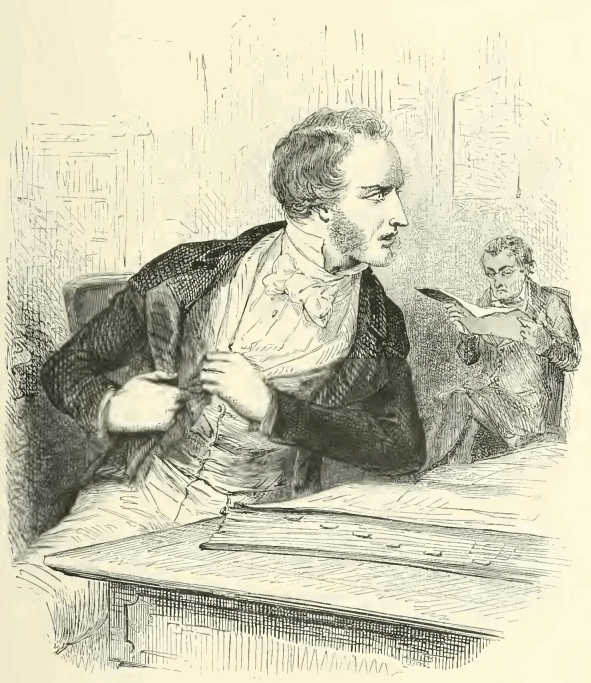
\includegraphics[width=\textwidth]{20029m.jpg}
\end{figure}

As to the note which accompanied this, the Englishman understood that
it might have been added by some inspector who had taken a momentary
interest in Dantès’ situation, but who had, from the remarks we have
quoted, found it impossible to give any effect to the interest he had
felt.

As we have said, the inspector, from discretion, and that he might not
disturb the Abbé Faria’s pupil in his researches, had seated himself in
a corner, and was reading \textit{Le Drapeau Blanc}. He did not see the
Englishman fold up and place in his pocket the accusation written by
Danglars under the arbor of La Réserve, and which had the postmark,
“Marseilles, 27th February, delivery 6 o’clock, P.M.”

But it must be said that if he had seen it, he attached so little
importance to this scrap of paper, and so much importance to his two
hundred thousand francs, that he would not have opposed whatever the
Englishman might do, however irregular it might be.

“Thanks,” said the latter, closing the register with a slam, “I have
all I want; now it is for me to perform my promise. Give me a simple
assignment of your debt; acknowledge therein the receipt of the cash,
and I will hand you over the money.”

He rose, gave his seat to M. de Boville, who took it without ceremony,
and quickly drew up the required assignment, while the Englishman
counted out the bank-notes on the other side of the desk.
